\documentclass[twoside,11pt,a4paper]{book}
\usepackage[amsbb]{mtpro2}
\usepackage[no-math,cm-default]{fontspec}
\usepackage{xunicode}
\usepackage{xgreek}
\defaultfontfeatures{Mapping=tex-text,Scale=MatchLowercase}
\def\xrwma{red!70!black}
\def\xrwmath{red!90!black}
\setmainfont[Mapping=tex-text,Numbers=Lining,Scale=1.0]{Minion Pro}
\newfontfamily\mpro{Minion Pro}
\usepackage{amsmath}
\usepackage[amsbb]{mtpro2}
\usepackage[left=2.00cm, right=2.00cm, top=3.00cm, bottom=2.00cm]{geometry}
\usepackage{makeidx}
\usepackage{longtable}
\usepackage{etoolbox}
\makeatletter
\newif\ifLT@nocaption
\preto\longtable{\LT@nocaptiontrue}
\appto\endlongtable{%
\ifLT@nocaption
\addtocounter{table}{\m@ne}%
\fi}
\preto\LT@caption{%
\noalign{\global\LT@nocaptionfalse}}
\makeatother
\makeindex
\usepackage{tikz,pgfplots}
\usepackage{tkz-euclide,tkz-fct}
\usepackage{wrapfig}
\usetkzobj{all}
\usepackage{calc}
\usepackage{cleveref}
\usepackage[colorlinks=false, pdfborder={0 0 0}]{hyperref}
\usepackage[framemethod=TikZ]{mdframed}
\newcommand{\ypogrammisi}[1]{\underline{\smash{#1}}}
\usetikzlibrary{backgrounds}
\renewcommand{\thepart}{\arabic{part}}
\definecolor{steelblue}{cmyk}{.7,.278,0,.294}
\definecolor{doc}{cmyk}{1,0.455,0,0.569}
\definecolor{olivedrab}{cmyk}{0.25,0,0.75,0.44}
\usepackage{capt-of}
\usepackage{titletoc}
\usepackage[explicit]{titlesec}
\usepackage{graphicx}
\usepackage{multicol}
\usepackage{multirow}
\usepackage{enumitem}
\usepackage{tabularx}
\usepackage{mathimatika,tkz-tab,gensymb}
\usepackage[decimalsymbol=comma]{siunitx}
\tikzset{>=latex}
\makeatletter
\pretocmd{\@part}{\gdef\parttitle{#1}}{}{}
\pretocmd{\@spart}{\gdef\parttitle{#1}}{}{}
\makeatother
\usepackage[titletoc]{appendix}
\usepackage{fancyhdr}
\pagestyle{fancy}
\fancyheadoffset{0cm}
\renewcommand{\headrulewidth}{\iftopfloat{0pt}{.5pt}}
\renewcommand{\chaptermark}[1]{\markboth{#1}{}}
\renewcommand{\sectionmark}[1]{\markright{\it\thesection\ #1}}
\fancyhf{}
\fancyhead[LE]{\thepage\ $\cdot$\ \scshape\nouppercase{\leftmark}}
\fancyhead[RO]{\nouppercase{\rightmark} $\cdot$\ \thepage}
\fancypagestyle{plain}{%
\fancyhead{} %
\renewcommand{\headrulewidth}{0pt}}

\newcounter{thewrhma}[chapter]
\renewcommand{\thethewrhma}{\thechapter.\arabic{thewrhma}} 
\newcommand{\Thewrhma}[1]{\refstepcounter{thewrhma}{\textbf{\textcolor{\xrwmath}{{\large Θεώρημα\hspace{2mm}\thethewrhma\;}:\;}\hspace{1mm}}} \MakeUppercase{\textbf{#1}}\\}{}

\newcounter{porisma}[chapter]
\renewcommand{\theporisma}{\thechapter.\arabic{porisma}}\newcommand{\Porisma}[1]{\refstepcounter{porisma}\textcolor{black}{\textbf{ΠΟΡΙΣΜΑ\hspace{2mm}\theporisma\hspace{1mm} \MakeUppercase{#1}}}\\}{}

\newcounter{protasi}[chapter]
\renewcommand{\theprotasi}{\thechapter.\arabic{protasi}}\newcommand{\Protasi}[1]{\refstepcounter{protasi}\textcolor{black}{\textbf{ΠΡΟΤΑΣΗ\hspace{2mm}\theprotasi\hspace{1mm} \MakeUppercase{#1}}}\\}{}

\newcounter{methodologia}[chapter]
\renewcommand{\themethodologia}{\thechapter.\arabic{methodologia}}\newcommand{\Methodologia}[1]{\refstepcounter{methodologia}\textcolor{black}{\textbf{MΕΘΟΔΟΣ\hspace{2mm}\themethodologia\hspace{1mm} \MakeUppercase{#1}}}\\}{}

\newcounter{orismos}[chapter]
\renewcommand{\theorismos}{\arabic{orismos}}   
\newcommand{\Orismos}[1]{\refstepcounter{orismos}{\textbf{\textbf{\textcolor{\xrwma}{{\large Ορισμός\hspace{2mm}\thechapter.\theorismos\;}:\;}}}}\hspace{1mm} \MakeUppercase{\textbf{#1}\\}}{}
\usepackage{venndiagram}
%-------- ΣΤΥΛ ΚΕΦΑΛΑΙΟΥ ---------
\newcommand*\chapterlabel{}
\newcommand{\fancychapter}{%
\titleformat{\chapter}
{
\normalfont\Huge}
{\gdef\chapterlabel{\thechapter\ }}{0pt}
{\begin{tikzpicture}[remember picture,overlay]
\node[yshift=-7cm] at (current page.north west)
{\begin{tikzpicture}[remember picture, overlay]
%\node[inner sep=0pt] at ($(current page.north) +			(0cm,-1.38in)$) {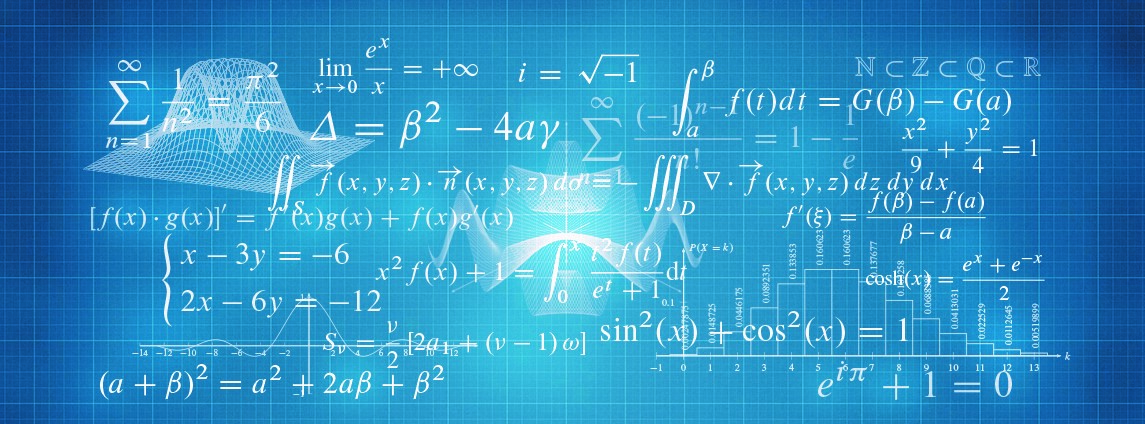
\includegraphics[width=17cm]{Kefalaio}};
\node[anchor=west,xshift=.08\paperwidth,yshift=.1\paperheight,rectangle]
{{\color{white}\fontsize{30}{20}\textbf{\textcolor{black}{\contour{white}{ΚΕΦΑΛΑΙΟ}}}}};
\node[anchor=west,xshift=.07\paperwidth,yshift=.05\paperheight,rectangle] {\fontsize{27}{20} {\color{black}{{\textcolor{black}{\contour{white}{\sc##1}}}}}};
%\fill[fill=black] (12.2,2) rectangle (14.8,4.7);
\node[anchor=west,xshift=.77\paperwidth,yshift=.077\paperheight,rectangle]
{\fontsize{80}{20}\textbf{\textit{\contour{black}{\thechapter}}}};
\end{tikzpicture}
};
\end{tikzpicture}
}
\titlespacing*{\chapter}{0pt}{20pt}{30pt}
}
%------------------------------------------------

\usepackage[outline]{contour}
\newcommand{\regularchapter}{%
\titleformat{\chapter}[display]
{\normalfont\huge\bfseries}{\chaptertitlename\ \thechapter}{20pt}{\Huge##1}
\titlespacing*{\chapter}
{0pt}{-20pt}{40pt}
}

\apptocmd{\mainmatter}{\fancychapter}{}{}
\apptocmd{\backmatter}{\regularchapter}{}{}
\apptocmd{\frontmatter}{\regularchapter}{}{}

\titlespacing*{\section}
{0pt}{30pt}{0pt}
\usepackage{booktabs}
\usepackage{hhline}
\DeclareRobustCommand{\perthousand}{%
\ifmmode
\text{\textperthousand}%
\else
\textperthousand
\fi}

\newcounter{typos}[chapter]
\renewcommand{\thetypos}{T\arabic{typos}}   
\newcommand{\Typos}{\refstepcounter{typos}\textcolor{gray}{\textbf{\thetypos}}}{}


\contentsmargin{0cm}
\titlecontents{part}[-1pc]
{\addvspace{10pt}%
\bf\Large ΜΕΡΟΣ\quad }%
{}
{}
{\;\dotfill\;\normalsize\ Σελίδα}%
%------------------------------------------
\titlecontents{chapter}[0pc]
{\addvspace{30pt}%
\begin{tikzpicture}[remember picture, overlay]%
\draw[fill=black,draw=black] (-.3,.5) rectangle (3.7,1.1); %
\pgftext[left,x=0cm,y=0.75cm]{\color{white}\sc\Large\bfseries Κεφάλαιο\ \thecontentslabel};%
\end{tikzpicture}\large\sc}%
{}
{}
{\hspace*{-2.3em}\hfill\normalsize Σελίδα \thecontentspage}%
\titlecontents{section}[2.4pc]
{\addvspace{1pt}}
{\contentslabel[\thecontentslabel]{2pc}}
{}
{\;\dotfill\;\small \thecontentspage}
[]
\titlecontents*{subsection}[4pc]
{\addvspace{-1pt}\small}
{}
{}
{\ --- \small\thecontentspage}
[ \textbullet\ ][]

\makeatletter
\renewcommand{\tableofcontents}{%
\chapter*{%
\vspace*{-20\p@}%
\begin{tikzpicture}[remember picture, overlay]%
\pgftext[right,x=12cm,y=0.2cm]{\Huge\sc\bfseries \contentsname};%
\draw[fill=black,draw=black] (9.5,-.75) rectangle (12.5,1);%
\clip (9.5,-.75) rectangle (15,1);
\pgftext[right,x=12cm,y=0.2cm]{\color{white}\Huge\bfseries \contentsname};%
\end{tikzpicture}}%
\@starttoc{toc}}
\makeatother
\pgfmathdeclarefunction{gauss}{2}{%
\pgfmathparse{1/(#2*sqrt(2*pi))*exp(-((x-#1)^2)/(2*#2^2))}%
}
\usepackage[contents={},scale=1,opacity=1,color=black,angle=0]{background}

\newcommand\blfootnote[1]{%
\begingroup
\renewcommand\thefootnote{}\footnote{#1}%
\addtocounter{footnote}{-1}%
\endgroup
}
\usepackage{epstopdf}
\epstopdfsetup{update}
\usepackage{textcomp}
\titleformat{\section}
{\normalfont\Large\bf}%
{}{0em}%
{{\color{black}\titlerule[1pt]}\vskip-.2\baselineskip{\parbox[t]{\dimexpr\textwidth-2\fboxsep\relax}{\raggedright\strut\thesection~#1\strut}}}[\vskip 0\baselineskip{\color{black}\titlerule[1pt]}]
\titlespacing*{\section}{0pt}{0pt}{0pt}

\newcommand{\methodologia}{\begin{center}
{\large \textbf{ΜΕΘΟΔΟΛΟΓΙΑ}}\\\vspace{-2mm}
\begin{tikzpicture}
\shade[left color=white, right color=black] (-3cm,0) rectangle (0,.2mm);
\shade[left color=black, right color=white] (0,0) rectangle (3cm,.2mm);   
\end{tikzpicture}
\end{center}}

\newcommand{\orismoi}{\begin{center}
\large \textcolor{\xrwma}{\textbf{ΟΡΙΣΜΟΙ}}\\\vspace{-2mm}
\begin{tikzpicture}
\shade[left color=white, right color=\xrwma] (-3cm,0) rectangle (0,.2mm);
\shade[left color=\xrwma, right color=white] (0,0) rectangle (3cm,.2mm);   
\end{tikzpicture}
\end{center}}
\newcommand{\thewrhmata}{\begin{center}
{\large \textcolor{\xrwmath}{\textbf{ΘΕΩΡΗΜΑΤΑ - ΠΟΡΙΣΜΑΤΑ - ΠΡΟΤΑΣΕΙΣ\\ΚΡΙΤΗΡΙΑ - ΙΔΙΟΤΗΤΕΣ}}}\\\vspace{-2mm}
\begin{tikzpicture}
\shade[left color=white, right color=\xrwmath,] (-5cm,0) rectangle (0,.2mm);
\shade[left color=\xrwmath, right color=white,] (0,0) rectangle (5cm,.2mm);   
\end{tikzpicture}
\end{center}}
\usepackage[labelfont={footnotesize,it,bf},font={footnotesize}]{caption}

\usepackage{wrapfig,wrap-rl}
%-------- ΜΑΘΗΜΑΤΙΚΑ ΕΡΓΑΛΕΙΑ ---------
\usepackage{mathtools}
%----------------------
%-------- ΠΙΝΑΚΕΣ ---------
\usepackage{booktabs}
%----------------------
%----- ΥΠΟΛΟΓΙΣΤΗΣ ----------
%\usepackage{calculator}
%----------------------------
\newcommand{\tss}[1]{\textsuperscript{#1}}
\newcommand{\tssL}[1]{\MakeLowercase{\textsuperscript{#1}}}
%----- ΟΡΙΖΟΝΤΙΑ ΛΙΣΤΑ ------
\usepackage{xparse}
\newcounter{answers}
\renewcommand\theanswers{\arabic{answers}}
\ExplSyntaxOn
\NewDocumentCommand{\results}{m}
{
\seq_set_split:Nnn \l_results_a_seq {,}{#1}
\par\nobreak\noindent\setcounter{answers}{0}
\seq_map_inline:Nn \l_results_a_seq
{
\makebox[.18\linewidth][l]{\stepcounter{answers}\theanswers.~##1}\hfill
}
\par
}
\seq_new:N \l_results_a_seq
\ExplSyntaxOff
%----------------------------

\usepackage{microtype}
\usepackage{float}
\usepackage{caption}
%----------- ΓΡΑΦΙΚΕΣ ΠΑΡΑΣΤΑΣΕΙΣ ---------
\pgfkeys{/pgfplots/aks_on/.style={axis lines=center,
xlabel style={at={(current axis.right of origin)},xshift=1.5ex, anchor=center},
ylabel style={at={(current axis.above origin)},yshift=1.5ex, anchor=center}}}
\pgfkeys{/pgfplots/grafikh parastash/.style={\xrwma,line width=.4mm,samples=200}}
\pgfkeys{/pgfplots/belh ar/.style={tick label style={font=\scriptsize},axis line style={-latex}}}
%-----------------------------------------

%---- ΟΡΙΖΟΝΤΙΟ - ΚΑΤΑΚΟΡΥΦΟ - ΠΛΑΓΙΟ ΑΓΚΙΣΤΡΟ ------
\newcommand{\orag}[3]{\node at (#1)
{$ \overcbrace{\rule{#2mm}{0mm}}^{{\scriptsize #3}} $};}

\newcommand{\kag}[3]{\node at (#1)
{$ \undercbrace{\rule{#2mm}{0mm}}_{{\scriptsize #3}} $};}

\newcommand{\Pag}[4]{\node[rotate=#1] at (#2)
{$ \overcbrace{\rule{#3mm}{0mm}}^{{\rotatebox{-#1}{\scriptsize$#4$}}}$};}
%-----------------------------------------
\tikzstyle{pl}=[line width=0.3mm]
\tikzstyle{plm}=[line width=0.4mm]
\tkzSetUpPoint[size=7,fill=white]
\newlist{rlist}{enumerate}{3}
\setlist[rlist]{itemsep=0mm,label=\roman*.}
\setlist[itemize]{itemsep=0mm}
\definecolor{bblue}{HTML}{4F81BD}
\definecolor{rred}{HTML}{C0504D}
\definecolor{ggreen}{HTML}{9BBB59}
\definecolor{ppurple}{HTML}{9F4C7C}

\makeatletter
\usetikzlibrary{patterns}
\tikzstyle{chart}=[
legend label/.style={font={\scriptsize},anchor=west,align=left},
legend box/.style={rectangle, draw, minimum size=5pt},
axis/.style={black,semithick,->},
axis label/.style={anchor=east,font={\tiny}},
]

\tikzstyle{bar chart}=[
chart,
bar width/.code={
\pgfmathparse{##1/2}
\global\let\bar@w\pgfmathresult
},
bar/.style={very thick, draw=white},
bar label/.style={font={\bf\small},anchor=north},
bar value/.style={font={\footnotesize}},
bar width=.75,
]

\tikzstyle{pie chart}=[
chart,
slice/.style={line cap=round, line join=round,thick,draw=white},
pie title/.style={font={\bf}},
slice type/.style 2 args={
##1/.style={fill=##2},
values of ##1/.style={}
}
]

\pgfdeclarelayer{background}
\pgfdeclarelayer{foreground}
\pgfsetlayers{background,main,foreground}


\newcommand{\pie}[3][]{
\begin{scope}[#1]
\pgfmathsetmacro{\curA}{90}
\pgfmathsetmacro{\r}{1}
\def\c{(0,0)}
\node[pie title] at (90:1.3) {#2};
\foreach \v/\s/\l in{#3}{
\pgfmathsetmacro{\deltaA}{\v/100*360}
\pgfmathsetmacro{\nextA}{\curA + \deltaA}
\pgfmathsetmacro{\midA}{(\curA+\nextA)/2}

\path[slice,\s] \c
-- +(\curA:\r)
arc (\curA:\nextA:\r)
-- cycle;
\pgfmathsetmacro{\d}{max((\deltaA * -(.5/50) + 1) , .5)}

\begin{pgfonlayer}{foreground}
\path \c -- node[pos=\d,pie values,values of \s]{$\l$} +(\midA:\r);
\end{pgfonlayer}

\global\let\curA\nextA
}
\end{scope}
}

\newcommand{\legend}[2][]{
\begin{scope}[#1]
\path
\foreach \n/\s in {#2}
{
++(0,-10pt) node[\s,legend box] {} +(5pt,0) node[legend label] {\n}
}
;
\end{scope}
}
\definecolor{a}{cmyk}{0,1,1,0.05}
\definecolor{b}{cmyk}{0,.8,.8,.15}
\definecolor{c}{cmyk}{0,.8,.8,.0}
\definecolor{d}{cmyk}{0,.7,.7,0}
\definecolor{e}{cmyk}{0,.5,.5,0}


\pgfplotsset{every axis/.append style={
x tick label style={/pgf/number format/.cd, 1000 sep={.}}}}
\newcommand{\shmeio}[2]{
\foreach \a in {1,...,#2}{
\node[dot] at (#1+.5,\a/2-.2){};}}





\begin{document}
\mainmatter
\pagestyle{fancy}
\chapter{Εξισώσεις - Ανισώσεις}
\section{Αλγεβρικές Παραστάσεις}\mbox{}\\
\orismoi
\Orismos{Μεταβλητή}
Μεταβλητή ονομάζεται το γράμμα ή το σύμβολο που χρησιμοποιούμε για να συμβολίσουμε έναν άγνωστο αριθμό. Χρησιμοποιούμε οποιοδήποτε γράμμα του ελληνικού ή του λατινικού αλφαβήτου όπως $ a,\beta,x,y,\ldots $\\\\
\Orismos{ΑΡΙΘΜΗΤΙΚΗ ΠΑΡΑΣΤΑΣΗ}
Αριθμητική ονομάζεται κάθε παράσταση η οποία περιέχει πράξεις μεταξύ αριθμών.\\\\
\Orismos{ΑΛΓΕΒΡΙΚΗ ΠΑΡΑΣΤΑΣΗ}
Αλγεβρική ονομάζεται κάθε παράσταση η οποία περιέχει πράξεις μεταξύ αριθμών και μεταβλητών.
\begin{itemize}[itemsep=0mm]
\item \textbf{Tιμή} μιας αλγεβρικής παράστασης ονομάζεται το αποτέλεσμα που προκύπτει ύστερα από πράξεις εαν αντικατασταθούν οι μεταβλητές της με αριθμούς.
\item Κάθε προσθετέος μέσα σε μια αλγεβρική παράσταση ονομάζεται \textbf{όρος} της παράστασης.
\end{itemize}
\Orismos{ΑΝΑΓΩΓΉ ΟΜΟΊΩΝ ΌΡΩΝ}
Αναγωγή ομοίων όρων ονομάζεται η διαδικασία με την οποία απλοποιούμε μια αλγεβρική παράσταση προσθέτοντας τoυς όμοιους όρους της.\\\\
\thewrhmata
\Thewrhma{Επιμεριστική Ιδιότητα}
Αν $ a,\beta,\gamma $ είναι τρεις οποιοιδήποτε αριθμοί τότε το γινόμενο του ενός με το άθροισμα των άλλων δίνεται από τον παρακάτω τύπο :
\[ a\cdot(\beta+\gamma)=a\cdot\beta+a\cdot\gamma \]
\section{Εξισώσεις}\mbox{}\\
\orismoi
\Orismos{Εξίσωση}
Εξίσωση ονομάζεται κάθε ισότητα που περιέχει τουλάχιστον μια μεταβλητή. Μια εξίσωση με έναν άγνωστο θα έιναι της μορφής :
\[ ax+\beta=0 \]
όπου $ a,\beta $ είναι οποιοιδήποτε αριθμοί.
\begin{itemize}[itemsep=0mm]
\item Μια εξίσωση αποτελείται από \textbf{2 μέλη}, τα οποία είναι τα μέρη της δεξιά και αριστερά του $ = $.
\[ \textrm{1ο μέλος}=\textrm{2ο μέλος} \]
\item \textbf{Άγνωστοι} ονομάζονται οι όροι της εξίσωσης οι οποίοι περιέχουν τη μεταβλητή, ενώ \textbf{γνωστοί} ονομάζονται οι αριθμοί δηλαδή οι σταθεροί όροι της εξίσωσης.
\item Κάθε αριθμός που επαληθεύει μια εξίσωση ονομάζεται \textbf{λύση} της εξίσωσης.
\item Η διαδικασία με την οποία βρίσκουμε τη λύση μιας εξίσωσης ονομάζεται \textbf{επίλυση}.
\item Εαν μια εξίσωση έχει λύσεις όλους τους πραγματικούς αριθμούς ονομάζεται \textbf{ταυτότητα} ή \textbf{αόριστη}.
\item Εαν μια εξίσωση δεν έχει καμία λύση ονομάζεται \textbf{αδύνατη}.
\end{itemize}
\Orismos{επαληθευση}
Επαλήθευση ονομάζεται η διαδικασία με την οποία εξετάζουμε αν ένας αριθμός είναι λύση μιας εξίσωσης, αντικαθιστώντας τη μεταβλητή της εξίσωσης με τον αριθμό αυτό.\\\\
\thewrhmata
\Thewrhma{Ιδιότητεσ ισοτήτων}
Σε κάθε ισότητα εαν τοποθετήσουμε τον ίδιο αριθμό και στα δύο μέλη της με πρόσθεση, αφαίρεση, πολλαπλασιασμό ή διαίρεση, η σχέση που προκύπτει είναι ξανά ισότητα :
\[ a=\beta\Rightarrow
\begin{cases}
a+\gamma=\beta+\gamma\\a-\gamma=\beta-\gamma
\end{cases}\ \ \textrm{ και }\ \ \begin{aligned}
&a\cdot\gamma=\beta\cdot\gamma\\&\dfrac{a}{\gamma}=\dfrac{\beta}{\gamma}\;\;,\;\;\gamma\neq0
\end{aligned} \]
\Thewrhma{Πράξεισ κατά μέλη}
Προσθέτοντας κατά μέλη κάθε ζεύγος ισοτήτων $ a=\beta $ και $ \gamma=\delta $ προκύπτει ισότητα, με 1\textsuperscript{ο} μέλος το άθροισμα των 1\textsuperscript{ων} μελών τους και 2\textsuperscript{ο} μέλος το άθροισμα των 2\textsuperscript{ων} μελών τους. Η ιδιότητα αυτή ισχύει και για αφαίρεση, πολλαπλασιασμό και διάιρεση κατά μέλη.
\[ \textrm{Αν }a=\beta\;\;\textrm{και}\;\;\gamma=\delta\Rightarrow\ccases{\textrm{\textbf{\textit{1. Πρόσθεση κατά μέλη }}}& a+\gamma=\beta+\delta\\\textrm{\textbf{\textit{2. Αφαίρεση κατά μέλη }}}& a-\gamma=\beta-\delta\\\textrm{\textbf{\textit{3. Πολλαπλασιασμός κατά μέλη }}}& a\cdot\gamma=\beta\cdot\delta\\\textrm{\textbf{\textit{4. \boldmath$ \varDelta $ιαίρεση κατά μέλη }}}& \dfrac{a}{\gamma}=\dfrac{\beta}{\delta}\;\;,\;\;\gamma\cdot\delta\neq0} \]
\section{Ανισώσεις}\mbox{}\\
\orismoi
\Orismos{Ανίσωση}
Ανίσωση ονομάζεται κάθε ανισότητα η οποία περιέχει τουλάχιστον μια μεταβλητή. Μια ανίσωση μιας μεταβλητής θα έχει τη μορφή
\[ ax+\beta>0\textrm{ ή }ax+\beta<0 \]
όπου $ a,\beta $ οποιοιδήποτε αριθμοί.
\begin{itemize}[itemsep=0mm]
\item Ανισώσεις αποτελούν και οι σχέσεις με σύμβολα ανισοϊσότητας $ \leq,\geq $.
\item Κάθε αριθμός που επαληθεύει μια ανίσωση ονομάζεται \textbf{λύση} της. Κάθε ανίσωση έχει λύσεις ένα \textbf{σύνολο αριθμών}.
\item Αν μια ανίσωση έχει λύσεις όλους τους αριθμούς ονομάζεται \textbf{αόριστη}.
\item Αν μια ανίσωση δεν έχει καθόλου λύσεις ονομάζεται \textbf{αδύνατη}.
\item Σχέσεις τις μορφής $ Q(x)\leq P(x)\leq R(x) $ λέγονται \textbf{διπλές ανισώσεις} όπου $ P(x),Q(x),R(x) $ είναι αλγεβρικές παρατάσεις. Αποτελείται από δύο ανισώσεις, με κοινό μέλος την παράσταση $ P(x) $, οι οποίες συναληθεύουν.
\item \textbf{Κοινές λύσεις} μιας διπλής ανίσωσης ή δύο ή περισσότερων ανισώσεων ονομάζονται οι αριθμοί που επαληθεύουν όλες τις ανισώσεις συγχρόνως.
\end{itemize}

\thewrhmata
\Thewrhma{ΙΔΙΟΤΗΤΕΣ ΑΝΙΣΟΤΗΤΩΝ}\label{th:idan}
\vspace{-5mm}
\begin{enumerate}
\item Εαν σε μια ανισότητα προσθέσουμε ή αφαιρέσουμε τον ίδιο αριθμό και απ' τα δύο μέλη της, προκύπτει ξανά ανισότητα με την ίδια φορά της αρχικής.
\[ a>\beta\Leftrightarrow\ccases{a+\gamma>\beta+\gamma\\a-\gamma>\beta-\gamma} \]
\item Για να πολλαπλασιάσουμε ή να διαιρέσουμε και τα δύο μέλη μιας ανισότητας με τον ίδιο αριθμό διακρίνουμε τις εξής περπτώσεις :
\begin{rlist}
\item Εαν πολλαπλασιάσουμε ή διαιρέσουμε και τα δύο μέλη μιας ανισότητας με τον ίδιο \textbf{θετικό} αριθμό, τότε προκύπτει ανισότητα με την \textbf{ίδια} φορά της αρχικής.
\item Εαν πολλαπλασιάσουμε ή διαιρέσουμε και τα δύο μέλη μιας ανισότητας με τον ίδιο \textbf{αρνητικό} αριθμό, τότε προκύπτει ανισότητα με φορά \textbf{αντίθετη} της αρχικής.
\end{rlist}
\begin{gather*}
\textrm{Αν }\gamma>0\textrm{ τότε }a>\beta\Leftrightarrow a\cdot\gamma>\beta\cdot\gamma\textrm{ και }\dfrac{a}{\gamma}>\dfrac{\beta}{\gamma}\\
\textrm{Αν }\gamma<0\textrm{ τότε }a>\beta\Leftrightarrow a\cdot\gamma<\beta\cdot\gamma\textrm{ και }\dfrac{a}{\gamma}<\dfrac{\beta}{\gamma}
\end{gather*}
\end{enumerate}
Ανάλογα συμπεράσματα ισχύουν και για τις ανισότητες $ a<\beta,a\geq\beta $ και $ a\leq\beta $.\\\\
\Thewrhma{Πράξεισ κατά μέλη ανισοτήτων}
Προσθέτοντας κατά μέλη κάθε ζεύγος ανισοτήτων προκύπτει ανισότητα, με 1\textsuperscript{ο} μέλος το άθροισμα των 1\textsuperscript{ων} μελών τους και 2\textsuperscript{ο} μέλος το άθροισμα των 2\textsuperscript{ων} μελών τους με φορά ίδια της αρχικής. Ομοίως πολλαπλασιάζοντας κατά μέλη δύο ανισότητες προκύπτει ανισότητα με φορά ίδια της αρχικής. Για να πολλαπλασιαστούν δύο ανισότητες κατά μέλη πρέπει όλοι οι όροι τους να είναι θετικοί.
\[ a>\beta\;\;\textrm{και}\;\;\gamma>\delta\Rightarrow\ccases{\textrm{\textbf{\textit{1. Πρόσθεση κατά μέλη }}}& a+\gamma>\beta+\delta\\\textrm{\textbf{\textit{2. Πολλαπλασιασμός κατά μέλη }}}& a\cdot\gamma>\beta\cdot\delta\;\;,\;\;\textrm{με }a,\beta,\gamma,\delta>0} \]
\textbf{Δεν} μπορούμε να αφαιρέσουμε ή να διαιρέσουμε ανισότητες κατά μέλη.\\\\
\chapter{Πραγματικοί Αριθμοί}
\section{Τετραγωνική ρίζα}\mbox{}\\
\orismoi
\Orismos{Τετραγωνική Ρίζα}
Τετραγωνική ρίζα ενός θετικού αριθμού $ x $ ονομάζεται ο \textbf{θετικός} αριθμός $ a $ που αν υψωθεί στο τετράγωνο δίνει τον αριθμό $ x $  και συμβολίζεται με $ \sqrt{x} $.
\[ \sqrt{x}=a\;\;,\;\;\textrm{ όπου }x\geq0\textrm{ και }a\geq0 \]
\begin{itemize}[itemsep=0mm]
\item Ο αριθμός $ x $ ονομάζεται \textbf{υπόριζο}.
\item Δεν ορίζεται ρίζα αρνητικού αριθμού.
\end{itemize}

\thewrhmata
\Thewrhma{Ιδιότητεσ Ριζών}
Για οποιουσδήποτε αριθμούς $ x,y $ ισχύουν οι παρακάτω ιδιότητες που αφορούν την τετραγωνική τους ρίζα.
\begin{center}
\begin{tabular}{cc}
\hline \rule[-2ex]{0pt}{5.5ex} \textbf{Ιδιότητα} & \textbf{Συνθήκη} \\
\hhline{==}\rule[-2ex]{0pt}{5.5ex}  Τετράγωνο ρίζας & $ \left(\sqrt{x}\;\right)^2=x\;\;,\;\; x\geq0  $ \\
\rule[-2ex]{0pt}{5.5ex}  Ρίζα τετραγώνου & $ \sqrt{x^2}=|x|\;\;,\;\;x\textrm{ πραγματικός}$\\
\rule[-2ex]{0pt}{5.5ex}  Ρίζα γινομένου & $ \sqrt{x\cdot y}=\!\sqrt{x}\cdot\!\sqrt{y}\;\;,\;\; x,y\geq0 $ \\
\rule[-2ex]{0pt}{6.5ex} Ρίζα πηλίκου & $ \sqrt{\dfrac{x}{y}}\;=\dfrac{\sqrt{x}}{\sqrt{y}}\;\;,\;\;x\geq0\textrm{ και }y>0 $\vspace{1mm} \\
\hline
\end{tabular}
\end{center}
Η ιδιότητα 3 ισχύει και για γινόμενο περισσότερων των δύο παραγόντων. \[ \sqrt{x_1\cdot x_2\cdot\ldots\cdot x_\nu}=\!\sqrt{x_1}\cdot\!\sqrt{x_2}\cdot\ldots\cdot\!\sqrt{x_\nu}\ \ ,\ \ x_1,x_2,\ldots x_\nu\geq0 \]
\section{Άρρητοι - Πραγματικοί αριθμοί}\mbox{}\\
\orismoi
\Orismos{Ρητός - άρρητος αριθμός}
Ρητός ονομάζεται ο αριθμός ο οποίος μπορεί να γραφτεί στη μορφή κλάσματος $ \frac{a}{\beta} $ με ακέραιους όρους $ a,\beta $. Κάθε αριθμός που δεν είναι ρητός ονομάζεται \textbf{άρρητος}.\\\\
\Orismos{Άξονασ των πραγματικών αριθμών}
Ο άξονας των πραγματικών αριθμών είναι μια αριθμημένη ευθεία στην οποία μπορούν να τοποθετηθούν όλοι οι πραγματικοί αριθμοί σε αύξουσα σειρά από τα αριστερά προς τα δεξιά. \textbf{Αρχή} του άξονα είναι το σημείο $ O $ στο οποίο βρίσκεται ο αριθμός $ 0 $.
\begin{center}
\begin{tikzpicture}
\tkzInit[xmin=-4,xmax=4]
\draw[-latex] (-5,0) -- coordinate (x axis mid) (5.4,0) node[right,fill=white] {{\footnotesize $ x $}};
\foreach \x in {-5,-4,-3,...,5}
\draw (\x,.5mm) -- (\x,-.5mm) node[anchor=north,fill=white] {{\scriptsize \x}};
\draw[latex-|] (-5,0.7) --  (-0.02,0.7);
\draw[|-latex] (0.02,0.7) --  (5,0.7);
\tkzText(-2,0.85){Αρνητικοί Αριθμοί}
\tkzText(2,0.85){Θετικοί Αριθμοί}
\tkzDefPoint(3,0){A}
\tkzDefPoint(1.4142,0){B}
\tkzDefPoint(-1.5,0){C}
\tkzDefPoint(-2.7,0){D}
\tkzDrawPoints[size=7,fill=white](A,B,C,D)
\tkzLabelPoint[above](A){{\scriptsize $ A(3) $}}
\tkzLabelPoint[above](B){{\scriptsize $ B\left(\!\! \sqrt{2}\right)  $}}
\tkzLabelPoint[above](C){{\scriptsize $ \varGamma\left(-\frac{3}{2} \right)  $}}
\tkzLabelPoint[above](D){{\scriptsize $ \varDelta(-2{,}7) $}}
\end{tikzpicture}
\end{center}
\begin{itemize}[itemsep=0mm]
\item Η θέση ενός αριθμού πάνω στην ευθεία σχεδιάζεται με ένα σημείο.
\item Ο αριθμός που βρίσκεται στη θέση αυτή ονομάζεται \textbf{τετμημένη} του σημείου.
\end{itemize}
\chapter{Συναρτήσεις}
\section{Η έννοια της συνάρτησης}\mbox{}\\
\orismoi
\Orismos{Συνάρτηση}
Συνάρτηση ονομάζεται μια σχέση που συνδέει δύο μεταβλητές $ x,y $ με την οποία \textbf{κάθε} τιμή της μεταβλητής $ x $ αντιστοιχεί σε \textbf{μια μόνο} τιμή της μεταβλητής $ y $.
\begin{itemize}[itemsep=0mm]
\item Κάθε συνάρτηση γράφεται σαν ισότητα η οποία περιέχει και τις δύο μεταβλητές. Η ισότητα αυτή λέγεται \textbf{εξίσωση} της συνάρτησης.
\item Αν $ y=A(x) $ όπου $ A(x) $ είναι μια αλγεβρική παράσταση του $ x $, τότε λέμε ότι η μεταβλητή $ y $ γραφεται \textbf{ως συνάρτηση} του $ x $.
\end{itemize}
\section{Γραφική παράσταση συνάρτησης}\mbox{}\\
\orismoi
\Orismos{Ορθογώνιο - Ορθοκανονικό Σύστημα Συντεταγμένων}
Ορθογώνιο σύστημα συντεταγμένων ονομάζεται το σχήμα που αποτελείται από δύο κάθετα τοποθετημένους μεταξύ τους άξονες αρίθμησης πάνω στους οποίους παίρνουν τιμές δύο μεταβλητές.
\begin{itemize}[itemsep=0mm]
\item Το σημείο τομής των δύο αξόνων ονομάζεται \textbf{αρχή των αξόνων}.
\item Σε κάθε άξονα του συστήματος, επιλέγουμε αυθαίρετα ένα μήκος το οποίο ορίζουμε ως μονάδα μέτρησης.
\item Εαν σε κάθε άξονα θέσουμε την ίδια μονάδα μέτρησης το σύστημα ονομάζεται \textbf{ορθοκανονικό}.
\item Ο οριζόντιος άξονας ονομάζεται \textbf{άξονας τετμημένων} και συμβολίζεται με $ x'x $.
\end{itemize}
\begin{minipage}{\linewidth}\mbox{}\\
\vspace{-1.2cm}
\begin{WrapText1}{10}{5cm}
\begin{tikzpicture}[scale=.48,y=1cm]
\tkzInit[xmin=-4,xmax=4.4,ymin=-4,ymax=4.4,ystep=1]
\draw[-latex]  (-4,0) node[left,fill=white] {{\footnotesize $ x' $}} -- coordinate (x axis mid) (4.4,0) node[right,fill=white] {{\footnotesize $ x $}};
\draw[-latex] (0,-4) node[below,fill=white] {{\footnotesize $ y' $}} -- (0,4.4) node[above,fill=white] {{\footnotesize $ y $}};
\draw (1,.15) -- (1,-.15) node[anchor=north] {\scriptsize 1};
\draw (.15,1) -- (-.15,1) node[anchor=east] {\scriptsize 1};
\tkzDefPoint(0,0){O}
\tkzDefPoint(2,1.8){M}
\tkzLabelPoint[below left](O){$ O $}
\tkzLabelPoint[right](M){{\footnotesize $ Μ(x,y) $}}
\draw[dashed] (0,1.8) node[left]{{\scriptsize $ y $}}--(2,1.8)--(2,0) node[below]{{\scriptsize $ x $}};
\tkzDrawPoint[size=7,fill=white](M)
\tkzText(2.2,3.3){{\scriptsize 1\textsuperscript{ο} Τεταρτημόριο}}
\tkzText(-2.2,3.3){{\scriptsize 2\textsuperscript{ο} Τεταρτημόριο}}
\tkzText(-2.2,-2){{\scriptsize 3\textsuperscript{ο} Τεταρτημόριο}}
\tkzText(2.2,-2){{\scriptsize 4\textsuperscript{ο} Τεταρτημόριο}}
\tkzText(2.2,2.7){{\scriptsize $ (+,+) $}}
\tkzText(-2.2,2.7){{\scriptsize $ (-,+) $}}
\tkzText(-2.2,-1.4){{\scriptsize $ (-,-) $}}
\tkzText(2.2,-1.4){{\scriptsize $ (+,-) $}}
\end{tikzpicture}
\end{WrapText1}
\begin{itemize}[itemsep=0mm]
\item Ο κατακόρυφος άξονας ονομάζεται \textbf{άξονας τεταγμένων} και συμβολίζεται με $ y'y $.
\item Κάθε σημείο του επιπέδου του συστήματος συντεταγμένων αντιστοιχεί σε ένα ζευγάρι αριθμών της μορφής $(x,y)$. Aντίστροφα, κάθε ζευγάρι αριθμών $(x,y)$ αντιστοιχεί σε ένα σημείο του επιπέδου.
\item Το ζεύγος αριθμών $(x,y)$ ονομάζεται \textbf{διατεταγμένο ζεύγος αριθμών} διότι έχει σημασία η διάταξη δηλαδή η σειρά με την οποία εμφανίζονται οι αριθμοί.
\item Οι αριθμοί $x,y$ ονομάζονται \textbf{συντεταγμένες} του σημείου στο οποίο αντιστοιχούν. Ο αριθμός $x$ ονομάζεται \textbf{τετμημένη} του σημείου ενώ ο $y$ \textbf{τεταγμένη}.
\end{itemize}\end{minipage}\mbox{}\\
\vspace{-2mm}
\begin{itemize}
\item Στον οριζόντιο άξονα $ x'x $, δεξιά της αρχής των αξόνων, βρίσκονται οι θετικές τιμές της μεταβλητής $x$ ενώ αριστερά, οι αρνητικές.
\item Αντίστοιχα στον κατακόρυφο άξονα $ y'y $, πάνω από την αρχή των αξόνων βρίσκονται οι θετικές τιμές της μεταβλητής $y$, ενώ κάτω οι αρνητικές τιμές.
\item Οι άξονες χωρίζουν το επίπεδο σε τέσσερα μέρη τα οποία ονομάζονται \textbf{τεταρτημόρια}. Ως 1\textsuperscript{ο} τεταρτημόριο ορίζουμε το μέρος στο οποίο ανήκουν οι θετικοί ημιάξονες $ Ox $ και $ Oy $.
\end{itemize}
\Orismos{Γραφική Παράσταση συνάρτησησ}
Γραφική παράσταση μιας συνάρτησης ονομάζεται το σύνολο των σημείων του επιπέδου $ M(x,y) $ των οποίων οι συντεταγμένες επαληθεύουν την εξίσωση της.\\
\begin{minipage}{\linewidth}\mbox{}\\
\vspace{-1.2cm}
\begin{WrapText1}{8}{4.7cm}
\vspace{-4mm}
\begin{tikzpicture}[scale=.7,domain=.2:4.5,y=.7cm]
\tkzInit[xmin=-.5,xmax=7,ymin=-.5,ymax=1.2,ystep=1]
\draw[-latex] (-.5,0) -- coordinate (x axis mid) (5,0) node[right,fill=white] {{\footnotesize $ x $}};
\draw[-latex] (0,-.5) -- (0,4.4) node[above,fill=white] {{\footnotesize $ y $}};
\draw[,domain=.3:3.7,samples=200,line width=.4mm,\xrwma] plot function{(x-2)**3-2*x+6};
\tkzDefPoint(1.5,2.875){A}
\tkzDrawPoint[size=7,fill=\xrwma,color=\xrwma](A)
\draw[dashed] (0,2.875) node[anchor=east]{{\scriptsize $ y $}}  -- (A) -- (1.5,0) node[anchor=north] {{\scriptsize $ x $}};
\tkzLabelPoint[above=1mm](A){{\footnotesize $ M\left( x,y\right)  $}}
\tkzDefPoint(0,0){O}
\tkzLabelPoint[below left](O){$ O $}
\end{tikzpicture}
\end{WrapText1}
\begin{itemize}[itemsep=0mm]
\item Το σύνολο των σημείων της παριστάνει σχήμα.
\item Η εξίσωση $ y=A(x) $ είναι η εξίσωση της γραφικής παραστασης την οποία επαληθεύουν οι συντεταγμένες των σημείων της.
\end{itemize}\end{minipage}\mbox{}\\\\\\
\section{Η συνάρτηση {$ \mathbold{y=ax} $}}\mbox{}\\
\orismoi
\Orismos{Η συνάρτηση \MakeLowercase{$ \mathbold{y=ax} $}}
\wrapr{-5mm}{7}{4cm}{-9mm}{\begin{tikzpicture}
\begin{axis}[x=1cm,y=.7cm,aks_on,xmin=-.5,xmax=3,
ymin=-.5,ymax=3,ticks=none,xlabel={\footnotesize $ x $},
ylabel={\footnotesize $ y $},belh ar]
\addplot[grafikh parastash,domain=-.5:2.7]{x};
\end{axis}
\node[fill=white,inner sep=.2mm] at (0.25,0.1) {$O$};
\node at (1.5,2) {{\footnotesize $y=ax$}};
\end{tikzpicture}}{
Η συνάρτηση $ y=ax $ είναι η συνάρτηση που συνδέει δύο \textbf{ανάλογα} ποσά $ x,y $.
\begin{itemize}[itemsep=0mm]
\item Η γραφική της παράσταση είναι ευθεία γραμμή η οποία διέρχεται από την αρχή των αξόνων.
\item Ο πραγματικός αριθμός $ a $ ονομάζεται \textbf{κλίση} της ευθείας. Ισούται με $ a=\frac{y}{x} $.
\end{itemize}}
\section{Η συνάρτηση {$ \mathbold{y=ax+\beta} $}}\mbox{}\\
\orismoi
\Orismos{Η συνάρτηση \MakeLowercase{$ \mathbold{y=ax+\beta} $}}
\wrapr{-5mm}{7}{4cm}{-9mm}{\begin{tikzpicture}
\begin{axis}[x=1cm,y=.7cm,aks_on,xmin=-.5,xmax=3,
ymin=-.5,ymax=3,ticks=none,xlabel={\footnotesize $ x $},
ylabel={\footnotesize $ y $},belh ar]
\addplot[grafikh parastash,domain=-.5:2.7,dashed]{x};
\addplot[grafikh parastash,domain=-.5:2]{x+1};
\end{axis}
\node[fill=white,inner sep=.2mm] at (0.25,0.1) {$O$};
\node at (1.5,2.5) {{\footnotesize $y=ax+\beta$}};
\draw[-latex] (1.5,1.05) -- (1.5,1.75);
\node at (1.35,1.35) {\footnotesize$\beta$};
\end{tikzpicture}}{
Η συνάρτηση $ y=ax+\beta $ παριστάνει ευθεία γραμμή η οποία είναι παράλληλη με την ευθεία $ y=ax $. \begin{itemize}[itemsep=0mm]
\item Ο αριθμός $ a $ ονομάζεται \textbf{κλίση} της ευθείας.
\item Η ευθεία $ y=ax+\beta $ με $ \beta\neq0 $ αποτελεί κατακόρυφη μετατόπιση της ευθείας $ y=ax $ ίση με $ \beta $ μονάδες.
\end{itemize}}
\thewrhmata
\Thewrhma{Η συνάρτηση \MakeLowercase{$ \mathbold{ax+\beta y=\gamma} $}}
Η εξίσωση $ ax+\beta y=\gamma $ παριστάνει ευθεία γραμμή αν ισχύει $ a\neq0 $ ή $ \beta\neq0 $.
\begin{itemize}[itemsep=0mm]
\item Οι εξισώσεις της μορφής $ y=\kappa $ παριστάνουν οριζόντιες ευθείες.
\item Οι εξισώσεις της μορφής $ x=\kappa $ παριστάνουν κατακόρυφες ευθείες.
\end{itemize}
\section{Η συνάρτηση {$ \mathbold{y=\frac{a}{x}} $}}\mbox{}\\
\orismoi
\Orismos{Η συνάρτηση \MakeLowercase{$ \mathbold{y=\frac{a}{x}} $}}
\wrapr{-5mm}{7}{4.5cm}{-10mm}{\begin{tikzpicture}
\begin{axis}[x=.7cm,y=.7cm,aks_on,xmin=-3,xmax=3,
ymin=-2.8,ymax=3,ticks=none,xlabel={\footnotesize $ x $},
ylabel={\footnotesize $ y $},belh ar]
\addplot[grafikh parastash,domain=.19:2.7]{.5/x};
\addplot[grafikh parastash,domain=-2.7:-.19]{.5/x};
\end{axis}
\node[fill=white,inner sep=.2mm] at (1.85,1.75) {$O$};
\node at (1.25,3) {$y=\frac{a}{x}$};
\end{tikzpicture}}{
Η συνάρτηση $ y=\frac{a}{x} $ είναι η συνάρτηση η οποία συνδέει δύο αντιστρόφως ανάλογα ποσά $ x,y $.
\begin{itemize}[itemsep=0mm]
\item Η γραφική της παράσταση ονομάζεται \textbf{υπερβολή}. Αποτελείται από δύο κλάδους όπως φαίνεται στο σχήμα.
\item Ο αριθμός $ a $ είναι διάφορος του μηδενός.
\end{itemize}}
\thewrhmata
\Thewrhma{Η συνάρτηση \MakeLowercase{$ \mathbold{y=\frac{a}{x}} $}}
Για τη γραφική παράσταση της συνάρτησης $ y=\frac{a}{x} $ ισχύουν τα εξής:
\begin{rlist}
\item Η υπερβολή έχει κέντρο συμμετρίας την αρχή των αξόνων.
\item Οι άξονες $ x'x $ και $ y'y $ είναι άξονες συμμετρίας της υπερβολής.
\item Αν $ a>0 $ η υπερβολή βρίσκεται στο 1\tss{ο} και στο 3\tss{ο} τεταρτημόριο ενώ αν $ a<0 $ βρίσκεται στο 2\tss{ο} και στο 4\tss{ο} τεταρτημόριο.
\end{rlist}
\begin{center}
\begin{tikzpicture}
\begin{axis}[x=.7cm,y=.7cm,aks_on,xmin=-3,xmax=3,
ymin=-2.8,ymax=3,ticks=none,xlabel={\footnotesize $ x $},
ylabel={\footnotesize $ y $},belh ar]
\addplot[grafikh parastash,domain=.19:2.7]{.5/x};
\addplot[grafikh parastash,domain=-2.7:-.19]{.5/x};
\end{axis}
\node[fill=white,inner sep=.2mm] at (1.85,1.75) {$O$};
\node at (1.25,3) {$y=\frac{a}{x}$};
\node at (1.25,2.5) {$a>0$};
\end{tikzpicture}\qquad\begin{tikzpicture}
\begin{axis}[x=.7cm,y=.7cm,aks_on,xmin=-3,xmax=3,
ymin=-2.8,ymax=3,ticks=none,xlabel={\footnotesize $ x $},
ylabel={\footnotesize $ y $},belh ar]
\addplot[grafikh parastash,domain=.19:2.7]{-.5/x};
\addplot[grafikh parastash,domain=-2.7:-.19]{-.5/x};
\end{axis}
\node[fill=white,inner sep=.2mm] at (1.85,1.75) {$O$};
\node at (3,3) {$y=\frac{a}{x}$};
\node at (3,2.5) {$a<0$};
\end{tikzpicture}
\end{center}
\end{document}